
\begin{figure}
    \centering
    \begin{subfigure}[c]{1.0\textwidth}
        \centering    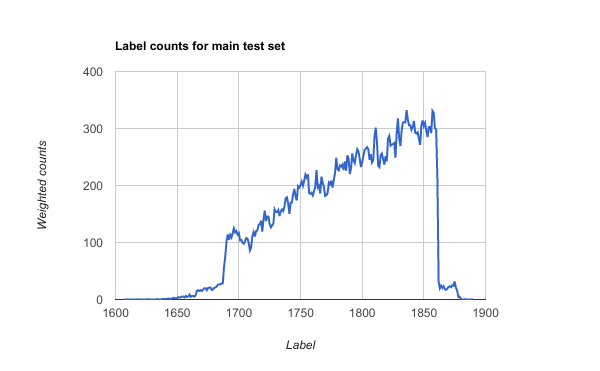
\includegraphics[scale=0.7]{resources/label_counts.png}
        \caption{Weighted label counts for the main training set and test set.}
        % \label{fig:mnist_early_models}
    \end{subfigure}
    
    \begin{subfigure}[c]{1.0\textwidth}
        \centering
        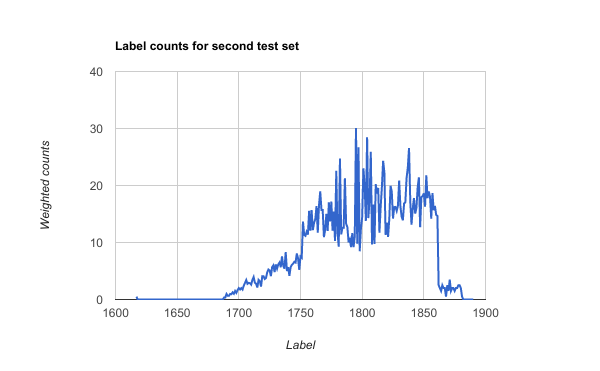
\includegraphics[scale=0.7]{resources/label_counts_sec.png}
        \caption{Weighted label counts for the second test set.}
        % \label{fig:mnist_models}
    \end{subfigure}
    
    \caption{Most pages come from the early 19th century, which is expected because of the population growth. However, there are very few pages after 1861.}
    \label{fig:label_counts}
\end{figure}
